\section{Inner Products and Norms}

Working a lot with $\R^2$ in this chapter, so there is geometry, which is easy to visualize.

\begin{definition}
  An \textbf{inner product} on $V$ is a function that takes each ordered pair $(u, v)$ of elements of $V$ to a number $\bangle{u, v} \in \F$ and has the following properties:
  \begin{itemize}
    \item positivity
          \begin{equation}
            \bangle{v, v} \geq 0, \forall v \in V
          \end{equation}
    \item definiteness
          \begin{equation}
            \bangle{v, v} = 0 \text{ iff } v = 0
          \end{equation}
    \item additivity in first slot
          \begin{equation}
            \bangle{u + v, w} = \bangle{u, w} + \bangle{v, w}, \forall u, v, w \in V
          \end{equation}
    \item homogeneity in first slot
          \begin{equation}
            \bangle{\lambda u, v} = \lambda \bangle{u, v}, \forall \lambda \in \F \text{ and all } u, v, w \in V
          \end{equation}
    \item conjugate symmetry
          \begin{equation}
            \bangle{u, v} = \conj{\bangle{v, u}}, \forall u, v \in V
          \end{equation}
  \end{itemize}
\end{definition}

\begin{theorem}
  Suppose $u, v \in V$. Then
  \begin{equation}
    \abs{
      \bangle{u, v}
    } \leq \norm{u}\norm{v}>
  \end{equation}
  The inequality is an equality iff one of $u, v$ is a scalar multiple of the other.
\end{theorem}

The Cauchy-Schwarz inequality is \textbf{very commonly used} in many parts of math, so I would pay attention to this and remember it!

\bx{
  I don't think additivity in first slot works
}

\bx{
  definiteness does not work, since we aren't considering the second coordinate.
}

\bx{
  not sure how to do this \TODO
}

\bx{
  \ea{
    \item We have
    \begin{align*}
      \bangle{u+v, u-v} & = \bangle{u, u-v} + \bangle{v, u-v}                                                \\
                        & = \bangle{u, u} - \bangle{u, v} + \bangle{v, u} - \bangle{v, v}                    \\
                        & = \norm{u}^2 - \norm{v}^2 \tag{Since $u, v$ real, $\bangle{v, u} = \bangle{u, v}$}
    \end{align*}
    \item From above, then the inner product is 0.
    \item The diagonals of a rhombus are $u+v, u-v$, and all sides are equal, so $\norm{u} = \norm{v}$.
  }
}

\bx{
  If $\norm{Tv} \leq \norm{v}$, then it must be the case that if there is an eigenvalue, then $\lambda \leq 1 < \sqrt{2}$, so thus we know $\sqrt{2}$ is not an eigenvalue and $T - \sqrt{2}I$ is invertible.
}

\bx{
  Forward direction is trivial, we just see $0 \leq X$ where $X$ is some inner product, which must be nonnegative.

  Backward direction we have
  \begin{align*}
    \norm{u}^2 & \leq \bangle{u+av, u+av}                                                      \\
               & \leq \bangle{u, u+av} + \bangle{av, u+av}                                     \\
               & \leq \conj{\bangle{u, u} + \bangle{av, u} + \bangle{u, av} + \bangle{av, av}} \\
    0          & \leq \conj{a}\bangle{u, v} + a\bangle{v, u} + \norm{a}^2\norm{v}^2            \\
               & \leq 2\Re(a\bangle{v, u}) + \norm{a}^2\norm{v}^2
  \end{align*}
  If we want this to hold $\forall a$, I think we need the real part to be zero, so we need $\bangle{v, u} = 0$? But this is not $\bangle{u, v}$.
}

\bx{
  \begin{align*}
    \norm{au + bv}^2
     & = \bangle{au +bv, au+bv}                                                                      \\
     & = a\bangle{u, au+bv} + b\bangle{v, au+bv}                                                     \\
     & = a\conj{\bangle{au+bv, u}} + b\conj{\bangle{au+bv, v}}                                       \\
     & = a\pa{
      \conj{a}\bangle{u, u} +
      \conj{b}\bangle{u, v}
    } + b\pa{
      \conj{a}\bangle{v, u} +
      \conj{b}\bangle{v, v}
    }                                                                                                \\
     & = a\conj{a}\norm{u}^2 + a\conj{b}\bangle{u, v} + b\conj{a}\bangle{v, u} + b\conj{b}\norm{v}^2
  \end{align*}
  \begin{align*}
    \norm{bu + av}^2
     & = \bangle{bu +av, bu+av}                                                                      \\
     & = b\bangle{u, bu+av} + a\bangle{v, bu+av}                                                     \\
     & = b\pa{
      \conj{b}\bangle{u, u} +
      \conj{a}\bangle{u, v}
    }
    + a\pa{
      \conj{b}\bangle{v, u} +
      \conj{a}\bangle{v, v}
    }                                                                                                \\
     & = a\conj{a}\norm{v}^2 + a\conj{b}\bangle{v, u} + b\conj{a}\bangle{u, v} + b\conj{b}\norm{u}^2
  \end{align*}
  If we have $\norm{u} = \norm{v}$, we just have to show
  \begin{align*}
    a\conj{b}\bangle{u, v} + b\conj{a}\bangle{v, u}
     & = a \conj{b}\bangle{v, u} + b\conj{a}\bangle{u, v}
  \end{align*}

  I might've missed something...don't think this should be this hard \TODO
}

\bx{
  \begin{align*}
    \abs{\bangle{u, v}} = 1
  \end{align*}
  means by the Cauchy-Schwarz inequality that $u = kv$. If we have that $\norm{u} = \norm{v} = 1$, then it must be the case that $k=1$, so we have $u = v$ as desired.
}

\bx{
  This is plug and chug Cauchy-Schwarz.
}

\bx{
  I think the system of equations to solve is
  \begin{align*}
    c & = \frac{
      \bangle{u, (1, 2)}
    }{5}                                         \\
    v & = u - \frac{\bangle{u, (1, 2)}}{5}(1, 2) \\
    u & = c(1, 2) + v
  \end{align*}
  The hardest part of the problem is re-assigning the variables from earlier ($u, v, w$) to the ones corresponding to this problem.
}

\bx{
  Let
  \begin{align*}
    u & = \pa{
      \sqrt{a}, \sqrt{b}, \sqrt{c}, \sqrt{d}
    }          \\
    v & = \pa{
      1/\sqrt{a}, 1/\sqrt{b}, 1/\sqrt{c}, 1/\sqrt{d}
    }
  \end{align*}
  and use the Cauchy-Schwarz inequality,
  \begin{align*}
    \abs{\bangle{u, v}} = \abs{
      1^2 + 1^2 + 1^2 + 1^2
    } = 4 & \leq \sqrt{
      a + b + c + d
    }\sqrt{
      1/a + 1/b + 1/c + 1/d
    } = \norm{u}\norm{v} \\
    16    & \leq \pa{
      a + b + c + d
    }\pa{
      1/a + 1/b + 1/c + 1/d
    } = \norm{u}\norm{v} \tag{square both sides}
  \end{align*}
}

\bx{
  This is just Cauchy-Schwarz with
  \begin{align*}
    u & = \pa{
      x_1, x_2, \dots, x_n
    }          \\
    v & = \pa{
      1, 1, \dots, 1
    } \tag{$n$ 1s}
  \end{align*}
}

\bx{
  Let's do some basic geometry
  \begin{figure}[H]
    \centering
    \begin{tikzpicture}
      \draw (0, 0) -- node[above] {$u$} ++(6, 4);
      \draw (0, 0) -- node[below] {$v$} ++(7, 2);
      \draw (6, 4) -- node[right] {$u-v$} (7, 2);
      \draw (1.5, 1) arc (20:3:1.81);
      \draw (1.5, 0.8) node[right] {$\theta$};
    \end{tikzpicture}
    \caption{Showing how to apply law of cosines.}
  \end{figure}
  By the law of cosines, this gives us
  \begin{align*}
    \norm{u-v}^2                                                         & = \norm{u}^2 + \norm{v}^2 - 2\norm{u}\norm{v}\cos\theta \\
    \bangle{u -v, u-v}  = \bangle{u, u} + \bangle{v, v} - 2\bangle{u, v} & = \norm{u}^2 + \norm{v}^2 - 2\norm{u}\norm{v}\cos\theta \\
    \bangle{u, v}                                                        & = \norm{u}\norm{v}\cos\theta
  \end{align*}
}

\bx{
  $\arccos$ is only defined with inputs $\in [-1, 1]$, so the Cauchy-Schwarz Inequality gives us this guarantee.
}

\bx{
  Pretty sure this is just Cauchy-Schwarz again. Whenever you see sums and inequalities, try Cauchy-Schwarz.
}

\bx{
  Let's draw this out,
  \begin{figure}[H]
    \centering
    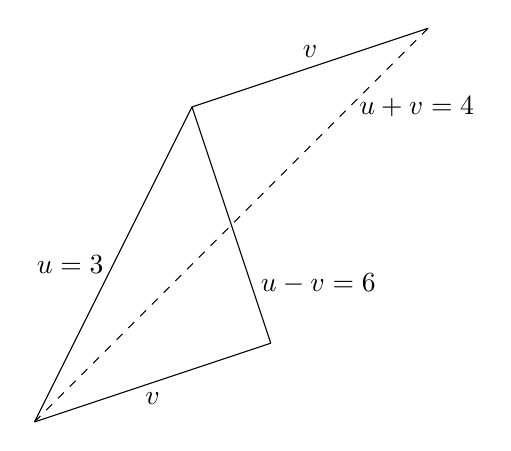
\begin{tikzpicture}
      \draw (0, 0) -- node[left] {$\norm{u} = 3$} ++(2, 4) -- node[above] {$v$} ++ (3, 1);
      \draw (0, 0) -- node[below] {$v$} ++(3, 1);
      \draw (2, 4) -- (2.5, 2.5) -- node[right] {$\norm{u-v} = 6$} (3, 1);
      \draw[dashed] (0, 0) -- (3, 3) -- node[right] {$\norm{u+v} = 4$} (5, 5);
    \end{tikzpicture}
    \caption{In geometry problems, always draw a good diagram.}
  \end{figure}
  Cool, so we have a parallelogram, so we can use 6.22 the parallelogram equality to give
  \begin{equation*}
    4^2 + 6^2 = 2(3^2 + \norm{v}^2) \implies \norm{v} = \sqrt{17}.
  \end{equation*}
}